\section{Даљински приступ меморији}
MPI-2 омогућава да процес директно приступи подацима другог процеса. Ове операције које омогућавају читање и писање тих података називају се \textit{remote memory access} (\gls{RMA}) операције. Главна карактеристика MPI имплементације је слање података између процеса помоћу операција за слање и примање података. 
Треба приметити да MPI-2 не омогућава реални подељени меморијски модел. Даљинске меморијске операције MPI-2 омогућавају велику флексибилност подељене меморије. 
Даљински приступ меморији је пројектован да ради на машинама са дељеном меморијом и на окружењима која немају дељену меморију, као што су мреже радних станица које користе TCP/IP протокол за комуникацију. Њихова главна предност је флексибилност коју нуде у пројектовању алгоритама. Крајњи програми су преносиви кроз све MPI имплементације и биће ефикасни на свим платформама које омогућавају приступ меморији других процеса.

\subsection{Меморијски оквири}

У строгом прослеђивању порука, бафери за слање и примање су одређени MPI типовима података који представљају делове адреса процеса који се шаљу другим процесима у случају слања, или адреса где ће други процеси уписати податке у случају примања. У MPI-2 имплементацији, појам комуникацијске меморије је генерализован на појам оквира за даљински приступ меморији. Сваки процес
може одредити део адресног простора који је доступан другим процесима за писање и читање. Операције писања и читања, које су покренуте од стране другог процеса називају се \textit{get} и \textit{put} операције за даљински приступ меморији(слика 3.6). Трећи тип операција је accumulate. У MPI-2, оквир представља део меморије једног процеса који чини дистрибуиран објекат, који се назива оквирни објекат. Оквирни објекат је направљен од више оквира, од којих се сваки састоји од локалне меморијске области која је изложена другим процесима.

\begin{figure}[h!]
  \centering
      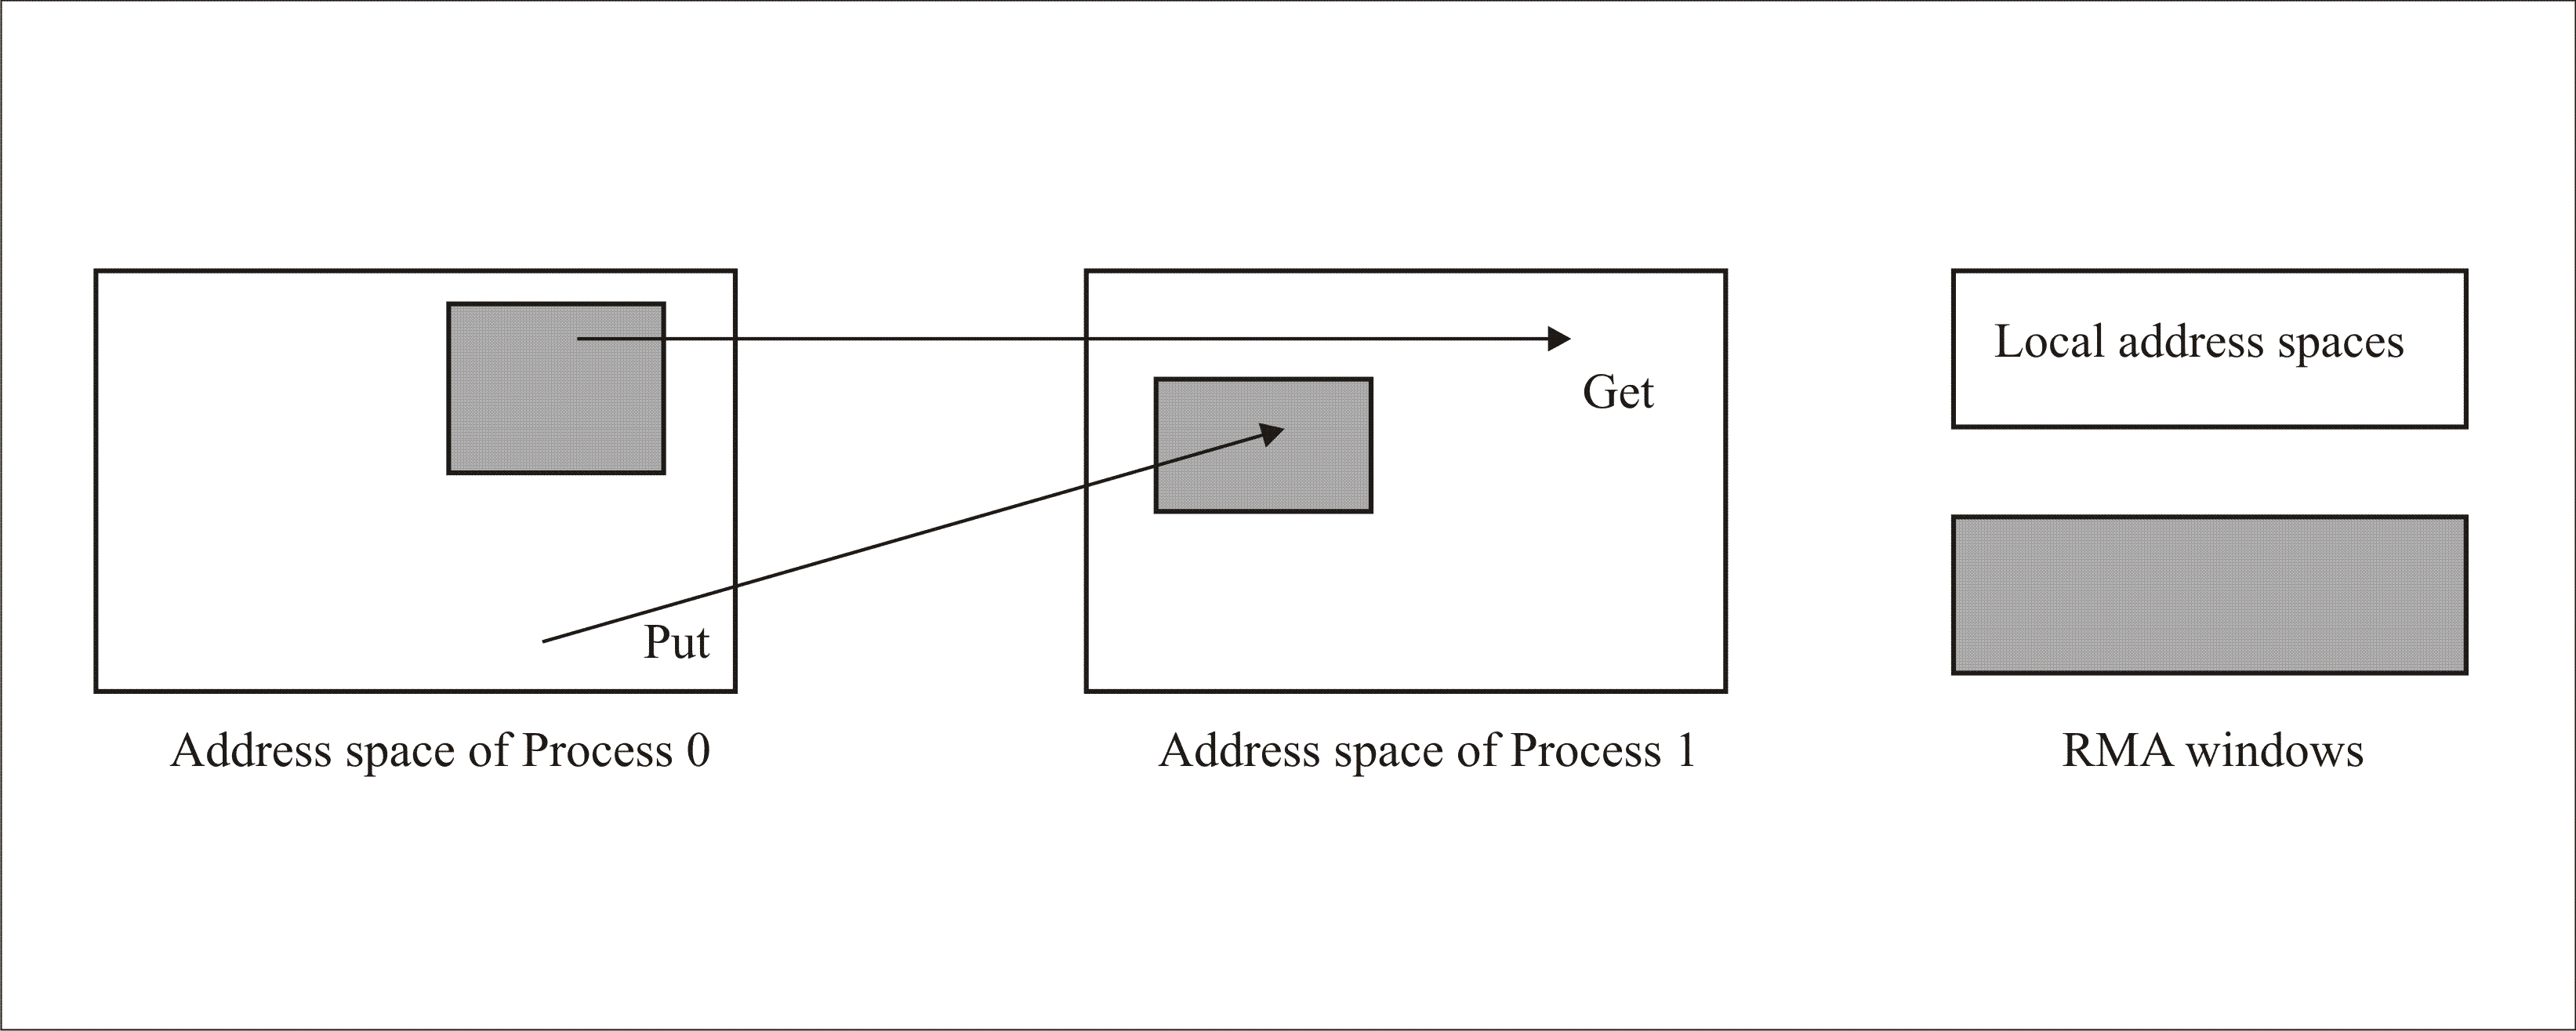
\includegraphics[width=1\textwidth]{slike/mpi_remote.png}
  \caption{Меморијски оквир}
\end{figure}

\subsection{Перформансе програма са даљинским приступом меморији}

Програм за рачунање $\pi$ рачуна вредност броја помоћу нумеричке интеграције. У класичној  верзији постоји 2 типа комуникације. Процес 0 комуницира са корисником и захтева број интервала за интеграцију. Помоћу функције \texttt{MPI\_Bcast} процес 0 шаље тај број другим процесима. Сваки процес затим израчунава парцијалну суму и све суме се сумирају помоћу колективне \texttt{MPI\_Reduce} операције.

У једностраној верзији овог програма, процес 0 снима вредност броја интервала као део RMA оквирног објекта, одакле га други процеси могу једноставно прочитати(Листинг 3.11). После израчунавања парцијалне суме, сви процеси додају своју вредност у други оквирни објекат помоћу accumulate операције. Сваки оквирни објекат садржи само један број у меморији. Оквирни објекти су представљени као променљиве типа \texttt{MPI\_Win}. Функције за креирање оквира су следеће:

\begin{verbatim}
	MPI_Win_create (&n, sizeof(int), 1, MPI_INFO_NULL, MPI_COMM_WORLD, &nwin);
	MPI_Win_create(MPI_BOTTOM, 0, 1, MPI_INFO_NULL, MPI_COMM_WORLD, &nwin);
\end{verbatim}

Позив са процеса 0 треба бити упарен са осталим процесима, иако они не доприносе никакву меморију за оквирни објекат, пошто је \texttt{MPI\_Win\_create} колективна операција над процесима који се налазе у комуникатору. Комуникатор одређује који процеси могу приступити оквирном објекту. Прва два аргумента функције  \texttt{MPI\_Win\_create} су адреса и дужина оквира у бајтовима.

\begin{lstlisting}[style=nonumbers,frame=single,language=C, caption=MPI програм са даљинским приступом меморији]
#include "mpi.h"
#include <math.h>

int main(int argc, char *argv[])
{
	int n, myid, numprocs, i;
	double PI25DT = 3.141592653589793238462643;
	double mypi, pi, h, sum, x;
	MPI_Win nwin, piwin;
	MPI_Init(&argc,&argv);
	MPI_Comm_size(MPI_COMM_WORLD,&numprocs);
	MPI_Comm_rank(MPI_COMM_WORLD,&myid);
	if (myid == 0)
	{
		MPI_Win_create(&n, sizeof(int), 1, MPI_INFO_NULL,
		MPI_COMM_WORLD, &nwin);
		MPI_Win_create(&pi, sizeof(double), 1, MPI_INFO_NULL,
		MPI_COMM_WORLD, &piwin);
	}
	else
	{
		MPI_Win_create(MPI_BOTTOM, 0, 1, MPI_INFO_NULL,
		MPI_COMM_WORLD, &nwin);
		MPI_Win_create(MPI_BOTTOM, 0, 1, MPI_INFO_NULL,
		MPI_COMM_WORLD, &piwin);
	}
	MPI_Win_fence(0, nwin);
	while (1)
	{
		if (myid == 0)
		{
			printf("Enter the number of intervals: (0 quits) ");
			fflush(stdout);
			scanf("%d",&n);
			pi = 0.0;
		}
		MPI_Win_fence(0, nwin);
		if (myid != 0)
		MPI_Get(&n, 1, MPI_INT, 0, 0, 1, MPI_INT, nwin);
		MPI_Win_fence(0, nwin);
		if (n == 0)
		{
			break;
		}
		else
		{
			h = 1.0 / (double) n;
			sum = 0.0;
			for (i = myid + 1; i <= n; i += numprocs)
			{
				x = h * ((double)i - 0.5);
				sum += (4.0 / (1.0 + x*x));
			}
			mypi = h * sum;
			MPI_Win_fence( 0, piwin);
			MPI_Accumulate(&mypi, 1, MPI_DOUBLE, 0, 0, 1, MPI_DOUBLE,
			MPI_SUM, piwin);
			MPI_Win_fence(0, piwin);
			if (myid == 0)
			printf("pi is approximately %. 16f, Error is %. 16f/n",
			pi, fabs(pi - PI25DT));
		}
	}
	MPI_Win_free(&nwin);
	MPI_Win_free(&piwin);
	MPI_Finalize();
	return 0;
}
\end{lstlisting}

Следећи аргумент је displacement unit који се користи да одреди одступање локације у меморији. Сваки оквирни објекат садржи једну променљиву, код којих је одступање нула, тако да одступање у овом примеру може да се занемари. Четврти аргумент је \texttt{MPI\_Info} који се може користити да побољша учинак RMA операција. Пети аргумент је комуникатор који одређује скуп процеса који ће имати приступ меморији оквирног објекта. MPI имплементација враћа \texttt{MPI\_Win} објекат као последњи аргумент. После позива функције \texttt{MPI\_Win\_create}, сваки процес који се налази у комуникатору има приступ
података \textit{nwin} помоћу операција \textit{put}, \textit{get} и \textit{accumulate}. За меморију оквира није потребно алоцирати посебну меморију, већ се користи меморија самог процеса, којој остали процеси приступају.  
MPI имплементација омогућава алоцирање посебне меморије позивом функције \texttt{MPI\_Alloc\_mem}.

Други позив функције \texttt{MPI\_Win\_create} креира оквирни објекат piwin дозвољавајући сваком процесу да приступи променљивој $\pi$ првог процеса, где ће бити смештена израчуната вредност броја $\pi$.
У следећем делу програма, процес са рангом 0 захтева број интервала, а затим остали процеси рачунају број $\pi$. Петља се завршава када корисник унесе нулу. Процеси којима ранг није нула, вредност броја $n$ узимају  директно из оквирног објекта без икакве додатне акције. Пре позива функције MPI\_Get или било које функције за даљински приступ меморији, потребно је позвати функцију \texttt{MPI\_Win\_fence} да одвоји операције. MPI имплементација омогућава специјални механизам синхронизације за операције дељене меморије - \textit{three of them}. \textit{Fence} операција је изазвана функцијом \texttt{MPI\_Win\_fence }која захтева два аргумента. Први аргумент је потврдни аргумент за дозвољавање оптимизације. Увек исправан потврдни аргумент је 0. Други аргумент је оквир на коме се операција извршава. \texttt{MPI\_Win\_fence} се може тумачити као баријера која одваја локалне операције на оквиру од скупа даљинских операција на оквиру.

У овом програму одваја читање вредности променљиве $n$ од осталих даљинских операција које следе. Вредност променљиве $n$ остали процеси добијају помоћу позивом:

\begin{verbatim}
MPI_Get(&n, 1, MPI_INT, 0, 0, 1, MPI_INT, nwin)
\end{verbatim}

Аргументи ове функције су слични аргументима функција које примају или шаљу податак. Get операција је слична операцији примања, па су зато прва три аргумента опис податка који се прима (адреса, количина и тип податка).  Следећи аргумент је ранг процеса чијој меморији приступамо. У овом случају је ранг 0, јер сви процеси приступају меморији првог процеса.
Следећа три аргумента дефинишу бафер за слање (адреса, количина и тип податка). Овде се адреса даје као одступање од почетка локације у дељеној меморији. У овом случају је 0, зато што се приступа само једној вредности. Последњи аргумент је објекат оквира.  \texttt{MPI\_Get} је неблокирајућа операција. После позива ове функције не може се гарантовати да је вредност смештена у променљивој $n$. Зато је потребно позвати \texttt{MPI\_Win\_fence}. Сваки процес рачуна свој део суме $mypi$. Сада се позива \texttt{MPI\_Win\_fence}, али на оквирном објекту piwin, како би се покренуо други 
RMA приступ. Позивом функције \texttt{MPI\_Accumulate}, сабирају се све суме процеса у глобалну суму.

\begin{verbatim}
MPI_Accumulate(&mypi, 1, MPI_DOUBLE, 0, 0, 1, MPI_DOUBLE, MPI_SUM, piwin)
\end{verbatim}

Прва три аргумента одређују локалну променљиву (адреса, количина и тип податка), док је четврти аргумент ранг процеса. Следећа три аргумента описују променљиву коју је потребно изменити.
Аргумент који следи је операција коју је потребно извршити. Пошто нам је потребна глобална сума, у овом случају то је \texttt{MPI\_SUM}. Последњи аргумент је објекат оквира.
Програм се завршава штампањем вредности броја $\pi$ и ослобађањем меморије објекта помоћу функције  \texttt{MPI\_Win\_free}.  \texttt{MPI\_Win\_free} је колективна функција над комуникатором прослеђеног објекта оквира.


Неке MPI функције у програмском језику C дате су у Листингу 3.12:

\begin{lstlisting}[style=nonumbers,frame=single,language=C, caption= MPI функције]
int MPI_Win_create(void *base, MPI_Aint size, int disp_unit, MPI_Info info,MPI_Comm comm, MPI_Win *win)
int MPI_Win_fence(int assert, MPI_Win win)
int MPI_Get(void *origin_addr, int origin_count, MPI_Datatype origin_datatype,
int target_rank, MPI_Aint target_disp, int target_count,
MPI_Datatype target_datatype, MPI_Win win)
int MPI_Accumulate(void *origin_addr, int origin_count,
MPI_Datatype origin_datatype, int target_rank,
MPI_Aint target_disp, int target_count,
MPI_Datatype target_datatype, MPI_Op op, MPI_Win win)
int MPI_Win_free(MPI_Win *win)
\end{lstlisting}

